
\chapter{小组总结}

\section{人员分工}

\begin{table}[h] %voc table result
	\centering
        \label{tab:glossary}
        \caption{小组成员分工表}
		\begin{tabular}{*{2}{c}}
			\toprule
	 		小组成员姓名 & 主要分工\\
            \midrule
            王永锋 & 项目管理,后端开发,编写API文档 \\
            张家豪 & 产品经理,编写规格说明书 \\
            何冠岚 & 后端开发,前端开发,美工设计 \\
            颜彬 & 前端开发,美工设计 \\
            李沐晗 & 编写单元测试 \\
			\bottomrule
		\end{tabular}
\end{table}



\section{项目特色}

本项目具有以下特色:

\begin{enumerate}
    \item \textbf{业界先进框架} \\ 前端采用基于 Vue.js 2.0 的桌面端组件库Element-UI, 后端采用基于Python3.6的Flask框架,数据库使用Mysql。
    \item \textbf{高效协同合作} \\ 使用Github进行项目管理,使用Swagger构建API文档,并采用API文档先行,前端,后端,单元测试同步开发的流程,确保开发效率。
    \item \textbf{项目质量保证} \\ 使用Travis-CI持续 集成工具对项目的每一次commit进行单元测试(单元测试使用pytest编写),测试成功后自动部署到服务器中。 通过自动化流程来使得软件构建、测试、发布更加快捷、频繁和可靠。
\end{enumerate}


\section{项目感想}

以前虽然也写过一些项目,但这一个项目,与以往的所有项目都有很大的不同。以前的项目总是有着一个明确的目标,完成实验要求即可,但这一个项目,我们没有任何明确的目标,也不清楚需要实现的产品。秉承着学习的心态,我们就选取了一个较为实际的问题,尝试了一些以前没有用过的框架以及工具,体验了一下之前没有经历过的开发流程,来让自己尽可能从这一个项目中能有更多的收获。

第一个体验的点是Github与项目管理。Github上的issue与pull request功能,让我们在解决项目遇到的问题时,有了一个反馈的渠道以及支持递进式迭代的更新方法。我们在提出需求,或者发现问题时,可以在Github上先提出一个issue,并且@对应负责的同学,此后该同学就可以在master分支上新开一个分支开发新的功能或者修复现有的bug,然后再通过提出pull request的方式,让项目的其他负责人对代码更改进行审核,审核通过后方可将代码合并到主分支中。

我们的代码分为三个仓库,主仓库为Waterfall\footnote{\url{https://github.com/wwyf/Waterfall}},前端代码所在仓库为\footnote{\url{https://github.com/YanB25/Waterfall-frontend}},后端代码所在仓库为\footnote{\url{https://github.com/wwyf/Waterfall-backend}}。得益于Github在项目管理上的优势,我们的每一行代码的改动都能够在Github找到相应的commit记录并得知对应的负责人,从而实现代码源头可追溯。同时,项目中曾出现过的bug,或者对一些实现细节的讨论,也在GitHub上得以永久存储。一些pull request的例子可见\autoref{fig:github_pull_resquest},更多的例子可在上面的各GitHub仓库中查看。

\begin{figure}[htp]
    %\begin{adjustwidth}{-1.5cm}{-1cm}
    \centering
    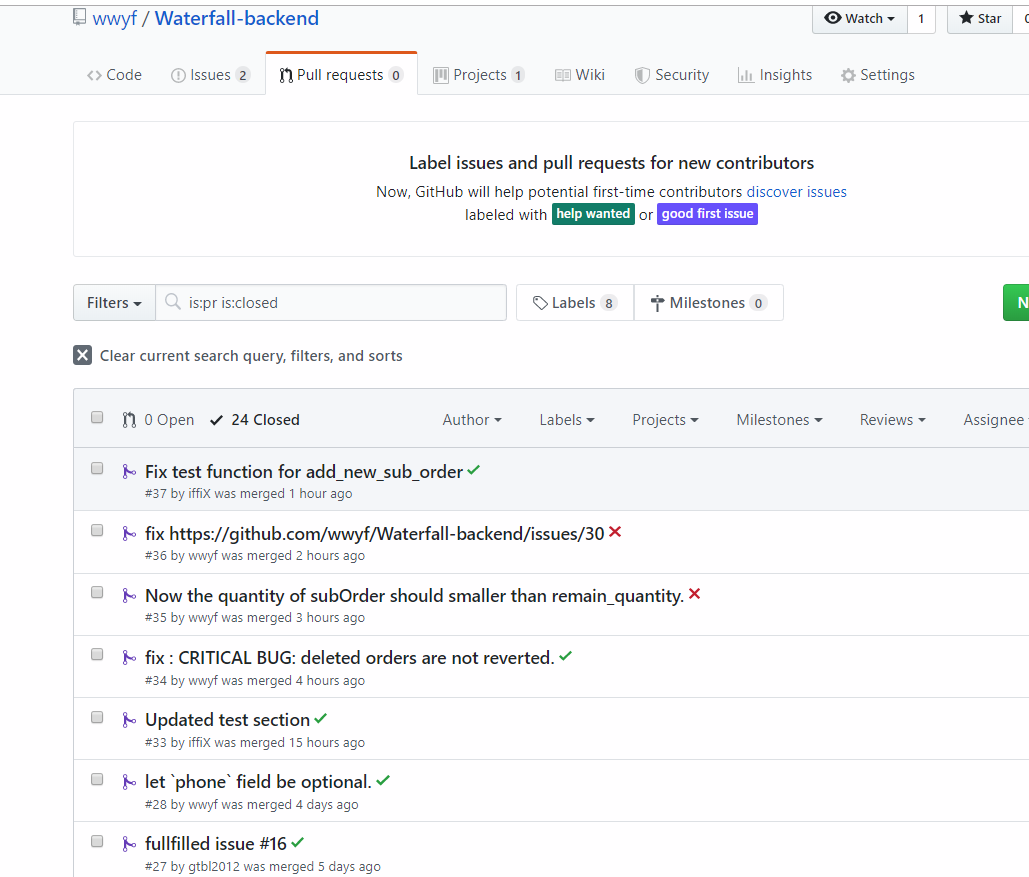
\includegraphics[width=12cm]{report/figure/appendix2/appendix2_github.png}
    \caption{Github中已解决的pull resquest例子}
    \label{fig:github_pull_resquest}
    %\end{adjustwidth}
\end{figure}

第二个体验的点是持续集成与自动部署。去年就听过老师讲解过DevOps的相关概念。DevOps(Development和Operations的组合词)是一组过程、方法与系统的统称,用于促进开发(应用程序/软件工程)、技术运营和质量保障(QA)部门之间的沟通、协作与整合。我们的开发过程虽然不敢说完全紧贴DevOps的业界实践,不过也尝鲜使用了Travis-CI持续集成工具来为我们组的软件开发添上些DevOps的风格。我们对代码的每一次更新,体现为GitHub仓库的每一次push,都会触发Travis-CI上的一次环境构建与单元测试。只有环境构建与单元测试皆通过了,才能够执行后面的部署步骤。基于此,我们便实现,对于代码的每一次push操作,都能够自动的完成构建,测试,部署流程,确保项目的开发质量与功能上线速度。

值得一提的是,我们的单元测试还使用了pytest-cov来进行代码覆盖度的计算。一次自动构建的例子\footnote{\url{https://travis-ci.org/wwyf/Waterfall-backend/builds/540797667}}可见\autoref{fig:travis-test1},一次自动测试的例子可见\autoref{fig:travis-test2},从中可见,代码覆盖度达到了100%。

\begin{figure}[htp]
    %\begin{adjustwidth}{-1.5cm}{-1cm}
    \centering
    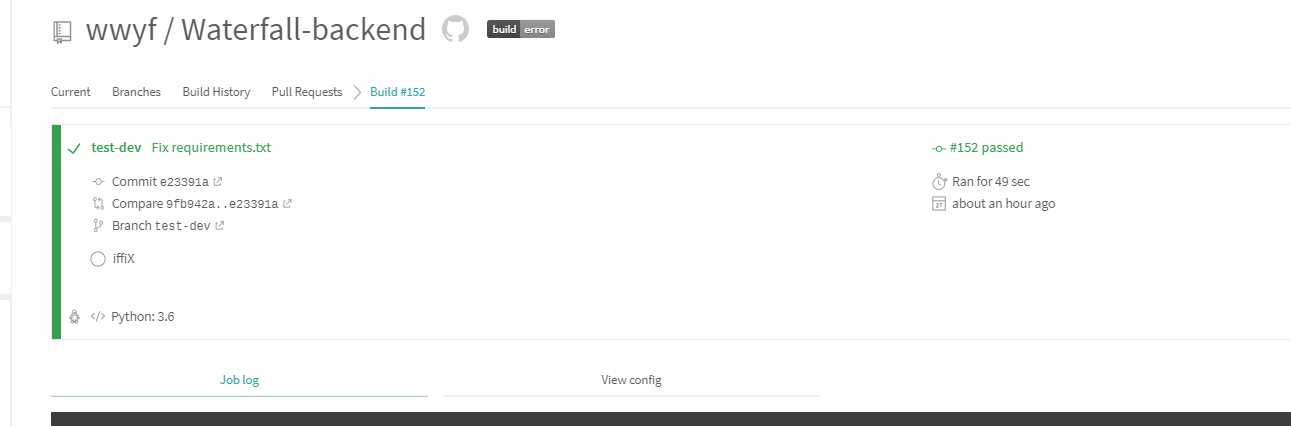
\includegraphics[width=13cm]{report/figure/appendix2/test1.png}
    \caption{Travis-CI持续集成}
    \label{fig:travis-test1}
    %\end{adjustwidth}
\end{figure}

\begin{figure}[htp]
    %\begin{adjustwidth}{-1.5cm}{-1cm}
    \centering
    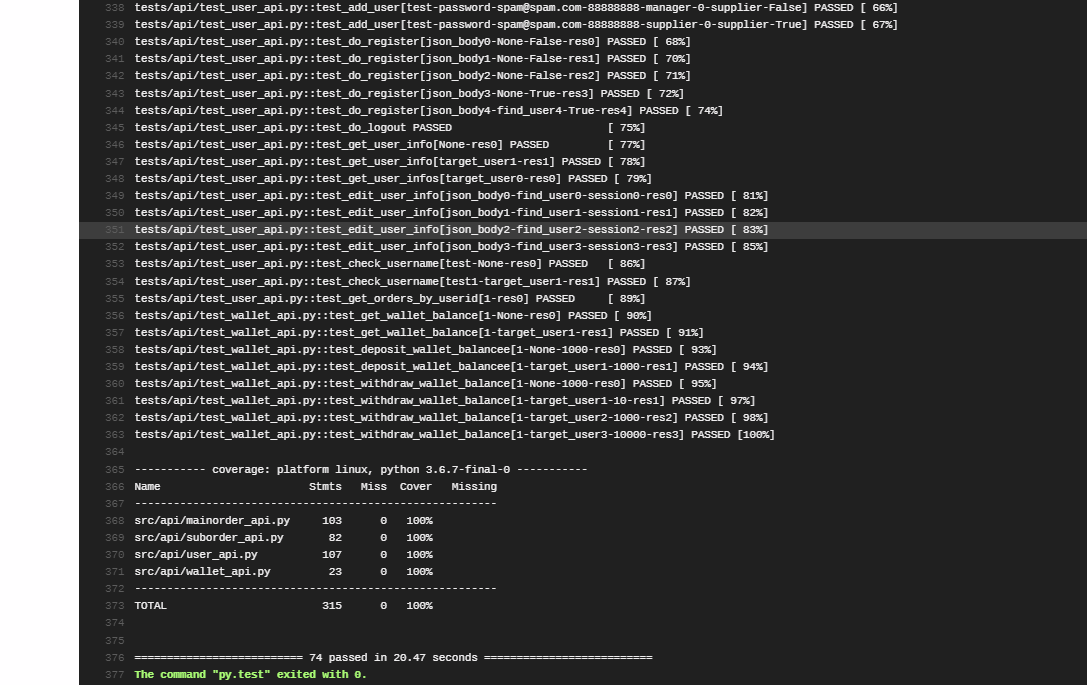
\includegraphics[width=13cm]{report/figure/appendix2/test2.png}
    \caption{Travis-CI自动测试}
    \label{fig:travis-test2}
    %\end{adjustwidth}
\end{figure}


第三个体验的点是docker化部署与微服务实践。得益于前后端分离的设计,我们的前端可以独立成一个docker用于提供http服务,后端也可以独立成一个用于处理用户逻辑的dockers容器,数据库更能独立成一个容器了。基于docker的设计,我们可以将应用和服务分解成更小的、松散耦合的组件,它们可以更加容易升级和扩展,并以可独立部署的服务套件发布,用户可根据成本以及性能要求将这些服务部署在一台服务器上或者分别部署在不同的服务器中。

\begin{figure}[htp]
    %\begin{adjustwidth}{-1.5cm}{-1cm}
    \centering
    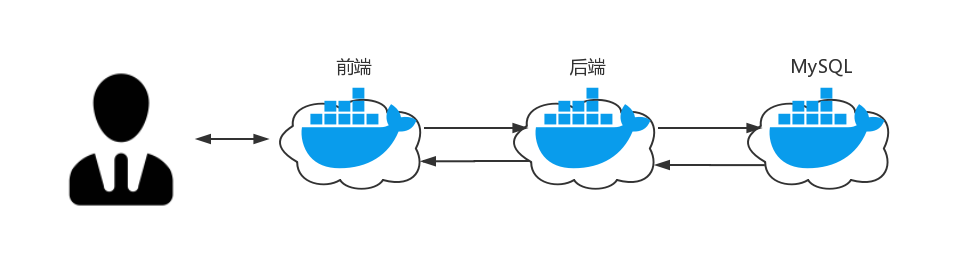
\includegraphics[width=15cm]{report/figure/appendix2/docker.png}
    \caption{微服务架构}
    \label{fig:docker}
    %\end{adjustwidth}
\end{figure}


当对系统性能要求不高时,我们可以使用如\autoref{fig:docker}所示的架构作为一个简单的微服务。若随着用户请求数增加,单个服务无法满足业务逻辑的处理要求时,系统可以采用对后端进行横向拓展的方式,可见\autoref{fig:docker2},分散业务逻辑的处理压力,充分利用云计算的优势,实现弹性伸缩。


\begin{figure}[htp]
    %\begin{adjustwidth}{-1.5cm}{-1cm}
    \centering
    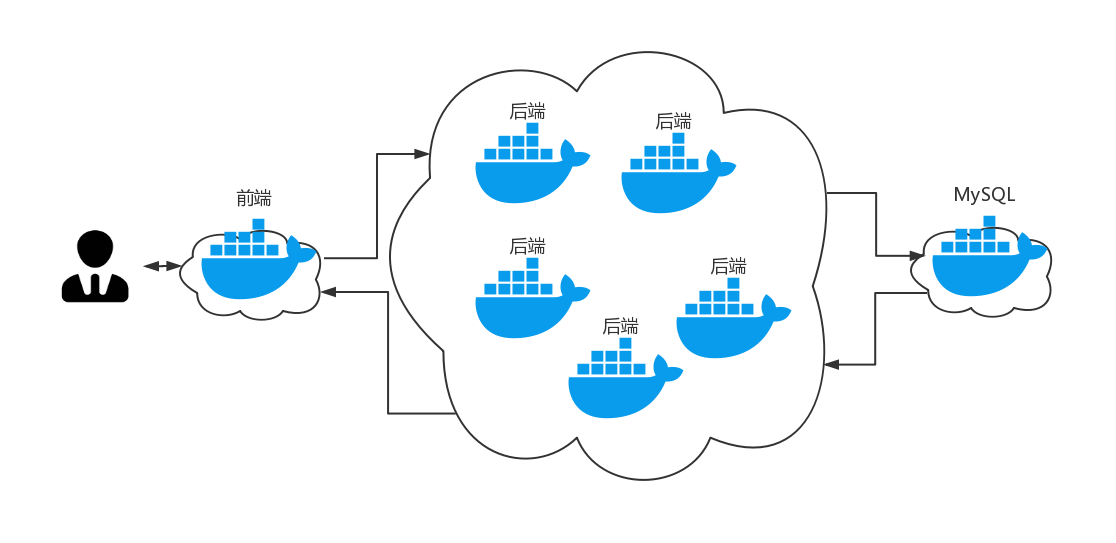
\includegraphics[width=15cm]{report/figure/appendix2/docker2.png}
    \caption{可横向扩展的微服务架构}
    \label{fig:docker2}
    %\end{adjustwidth}
\end{figure}


第四个体验的点是前后端高度分离与API文档的设计。为了达成前后端分离的目的,我们必须以一个高度明确的API文档来对前后端之间交互的接口进行明确清晰的定义。我们首先基于OpenAPI3.0规范,编写了API文档,并使用Swagger工具\footnote{该工具部署在了我们小组的服务器上,链接为\url{https://swagger.ui.wwyf.top}},将API文档以网页的形式清晰的展现出来,对接口接受与返回的每一个字段都进行明确的定义的说明,如\autoref{fig:swagger_api}所示,方便前端、后端、测试同时针对此接口同时进行开发。

\begin{figure}[htp]
    %\begin{adjustwidth}{-1.5cm}{-1cm}
    \centering
    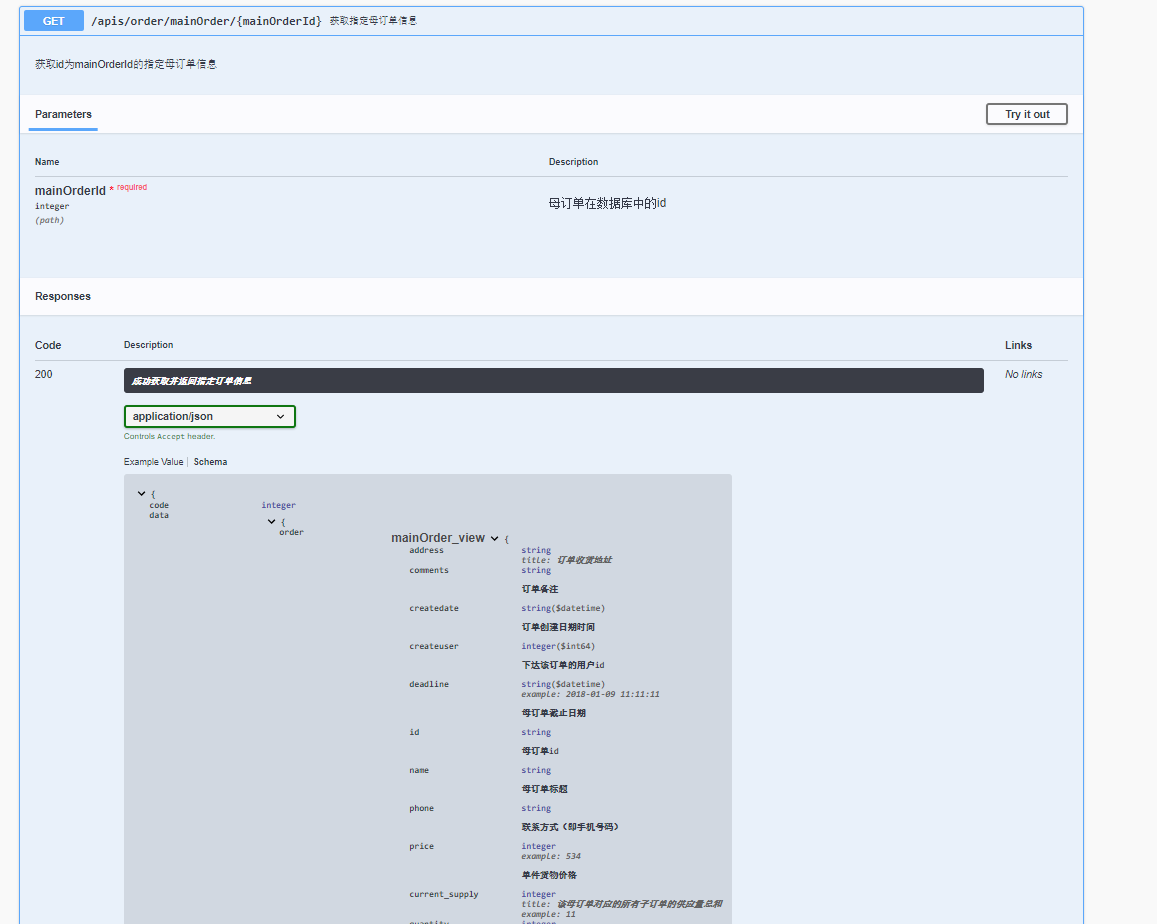
\includegraphics[width=15cm]{report/figure/appendix2/swagger_api.png}
    \caption{Sqagger可视化的API文档示例}
    \label{fig:swagger_api}
    %\end{adjustwidth}
\end{figure}

除此之外,我们还从中学到了很多有关前后端开发中与框架相关的知识,无论是Element-UI还是Flask,都是目前业界中广泛使用的框架,我们在使用这些框架进行开发时,也学习到了不少优秀项目使用的开发风格,并应用到我们的项目中。

总而言之,无论在该系统的设计,开发,测试,还是维护,软件工程的方法论无处不在,处处皆有体现,我们也在该项目中受益良多。这些收获将对自己的能力有进一步的提升,更在之后的开发中渐渐体现其价值所在!


\section{项目代码仓库链接}

本项目中所使用的三个代码仓库可见\autoref{tab:github}

\begin{table}[h] %voc table result
	\centering
        \caption{项目代码仓库链接表}
        \label{tab:github}
		\begin{tabular}{*{3}{c}}
			\toprule
	 		仓库名称 & 仓库作用  & 链接\\
            \midrule
            Waterfall & 规格说明书 & \url{https://github.com/wwyf/Waterfall} \\
            Waterfall-backend & 后端代码 & \url{https://github.com/wwyf/Waterfall-backend} \\
            Waterfall-frontend & 前端代码 & \url{https://github.com/YanB25/Waterfall-frontend} \\
			\bottomrule
		\end{tabular}
\end{table}


\endinput
